\documentclass[12pt]{article}

\usepackage[a4paper,margin=2cm]{geometry}

\usepackage{amsmath}
\usepackage{amssymb}
\usepackage{mathtools}

\usepackage{listings}

\usepackage{booktabs} % For tables
\usepackage[table,xcdraw]{xcolor} % For tables

\usepackage{tikz} % TikZ

\usepackage{enumerate}
\usepackage{enumitem}

\usepackage{nameref}

\usepackage{xcolor}

\definecolor{codegreen}{rgb}{0,0.6,0}
\definecolor{codegray}{rgb}{0.5,0.5,0.5}
\definecolor{codepurple}{rgb}{0.58,0,0.82}
\definecolor{backcolour}{rgb}{0.95,0.95,0.92}

\lstdefinestyle{mystyle}{
    backgroundcolor=\color{backcolour},
    commentstyle=\color{codegreen},
    keywordstyle=\color{magenta},
    numberstyle=\tiny\color{codegray},
    stringstyle=\color{codepurple},
    basicstyle=\ttfamily\footnotesize,
    breakatwhitespace=false,
    breaklines=true,
    captionpos=b,
    keepspaces=true,
    numbers=left,
    numbersep=5pt,
    showspaces=false,
    showstringspaces=false,
    showtabs=false,
    tabsize=2
}

\lstset{style=mystyle}

\DeclarePairedDelimiter\abs{\lvert}{\rvert}
\DeclarePairedDelimiter\Abs{\lVert}{\rVert}

\usepackage{fancyhdr}

\pagestyle{fancy}
\lhead{\today}
\chead{Exercise 04\\Algorithmic Foundations of Data Science}
\rhead{Fabian Grob\\Simon Michau\\Til Mohr}

\setlength{\headheight}{50pt}

\begin{document}

\section*{Exercise 1}
\subsection*{(a)}
Situation for l=2 and s=2:
\[Q_{2,2}=\lbrace [x_1 x_2]^T\in\mathbb{R}^2\mid |x_i|\leq 1 \text{ for all } i=1,2\rbrace = [-1,1]^2\]
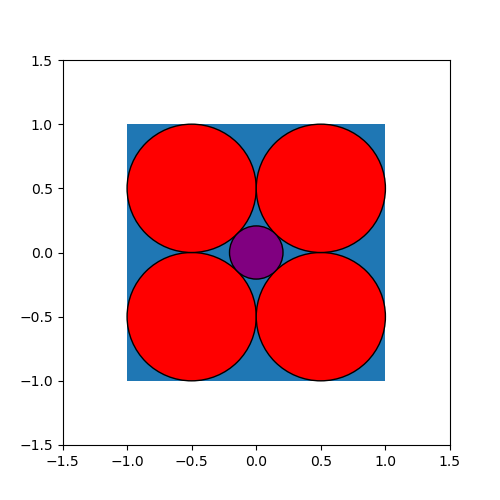
\includegraphics[width=3.5in]{code/exercise_01_a.png}
\subsection*{(b)}

\section*{Exercise 2}
\subsection*{(a)}
\subsection*{(b)}

\section*{Exercise 3}
\subsection*{(a)}
\subsection*{(b)}
\subsection*{(c)}
\subsection*{(d)}

\section*{Exercise 4}
\subsection*{(a)}
\subsection*{(b)}
\subsection*{(c)}
\subsection*{(d)}
\subsection*{(e)}

\section*{Exercise 5}


\end{document}